\chapter{Experiment}
\section{Slab Waveguide}



\section{Quadratic single-mode strip waveguide}
\label{sec:task2}

The next step was to simulate a three dimensional strip waveguide in air with a higth and a lenght of 0.356~$upmu$m and a core refractive index $n$~=~3.03 in air.
The lenght of the waveguide was 100~$\upmu$m.

Figure \ref{fig:2_index} shows the index profile of the waveguide.
% 
% \begin{figure}%
% 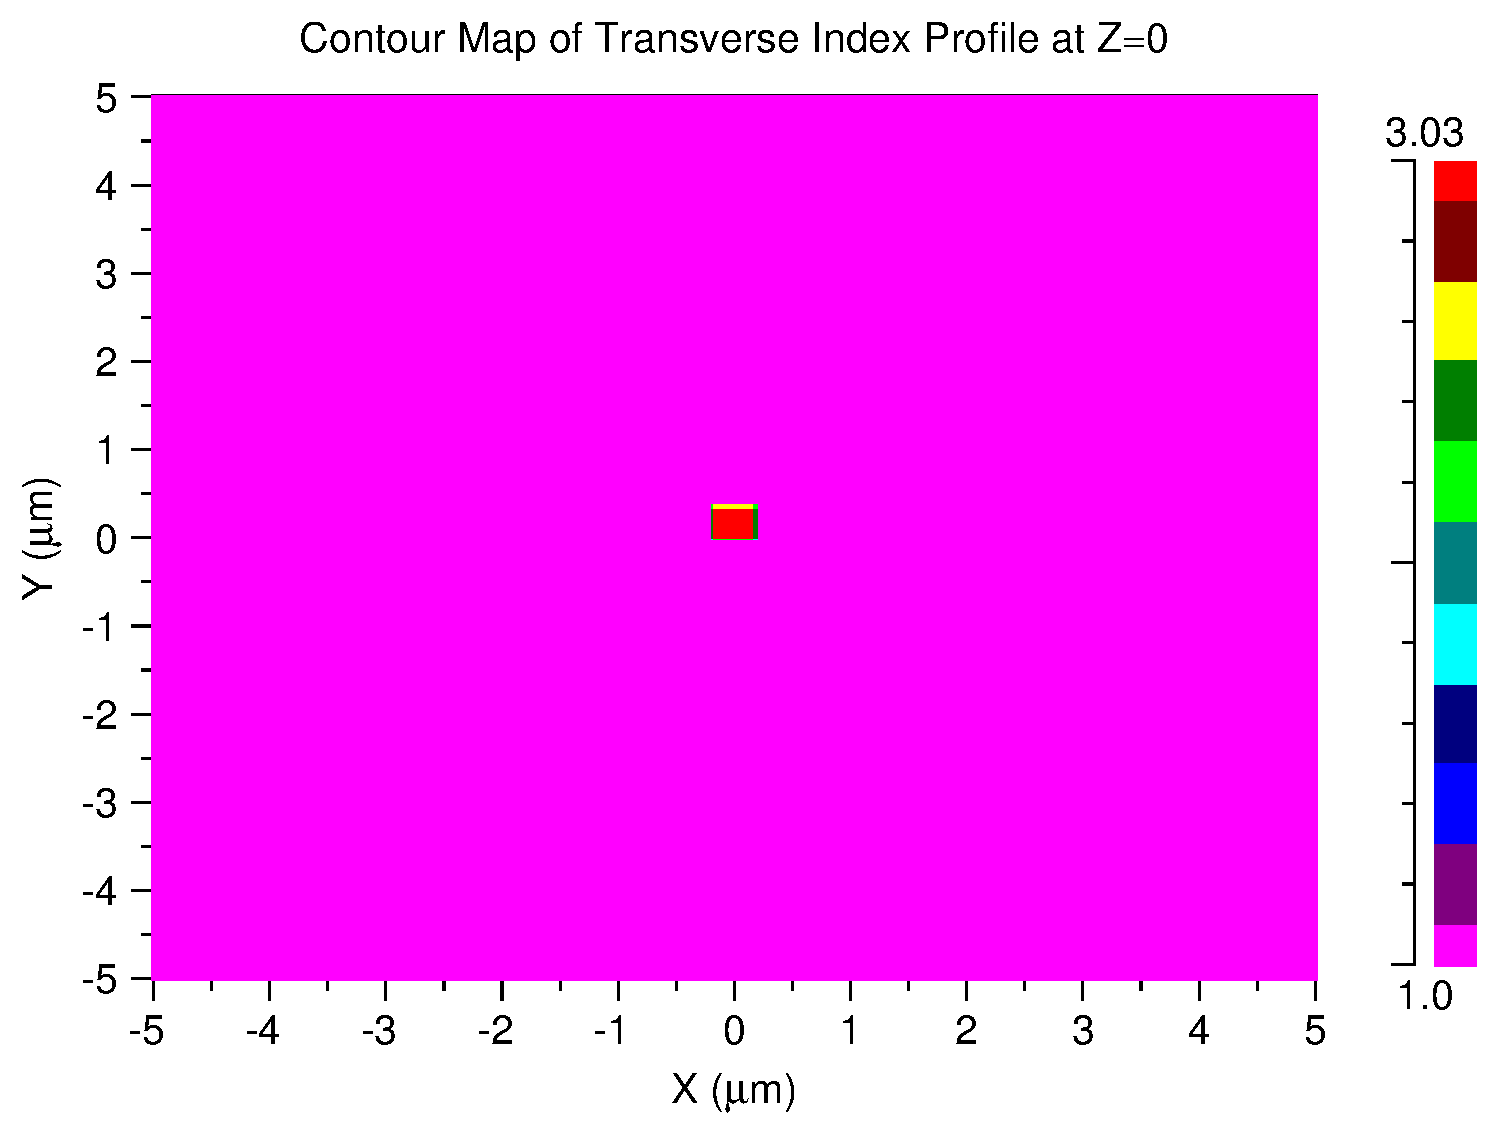
\includegraphics[width=.5\columnwidth]{Grafiken/2_index}%
% \caption{index profile of the quadratic single-mode strip waveguide.}%
% \label{fig:2_index}%
% \end{figure}

The excitation of the field is Gaussian and and has an offset in x direction by 0.25 times the width and in y direction by 0.25 times the hight of the waveguide.
For this waveguide all modes wer calculated at a frequency of 200~THz by using the correlation method and a grid size in x/y/z-direction of 0.02/0.02/0.05. 


% 
% \begin{figure}%
% \centering
% %\begin{adjustwidth}{0cm}{0cm}
% 	\subfloat[  ]{\includegraphics[totalheight=6 cm]{Grafiken/  }\label{fig:}}
% 	\subfloat[  ]{\includegraphics[totalheight=4 cm]{Grafiken/  } \label{fig:  }}\\%
% 	\subfloat[  ]{\includegraphics[totalheight=4 cm]{Grafiken/  }\label{fig:  }}
% 	\subfloat[  ]{\includegraphics[totalheight=4 cm]{Grafiken/  } \label{fig:  }}
% %\end{adjustwidth}
% \caption{}%
% \label{fig:2_modes}%
% \end{figure}




\section{Design of a SOI strip waveguide}

\begin{figure}%
\centering
%\begin{adjustwidth}{0cm}{0cm}
 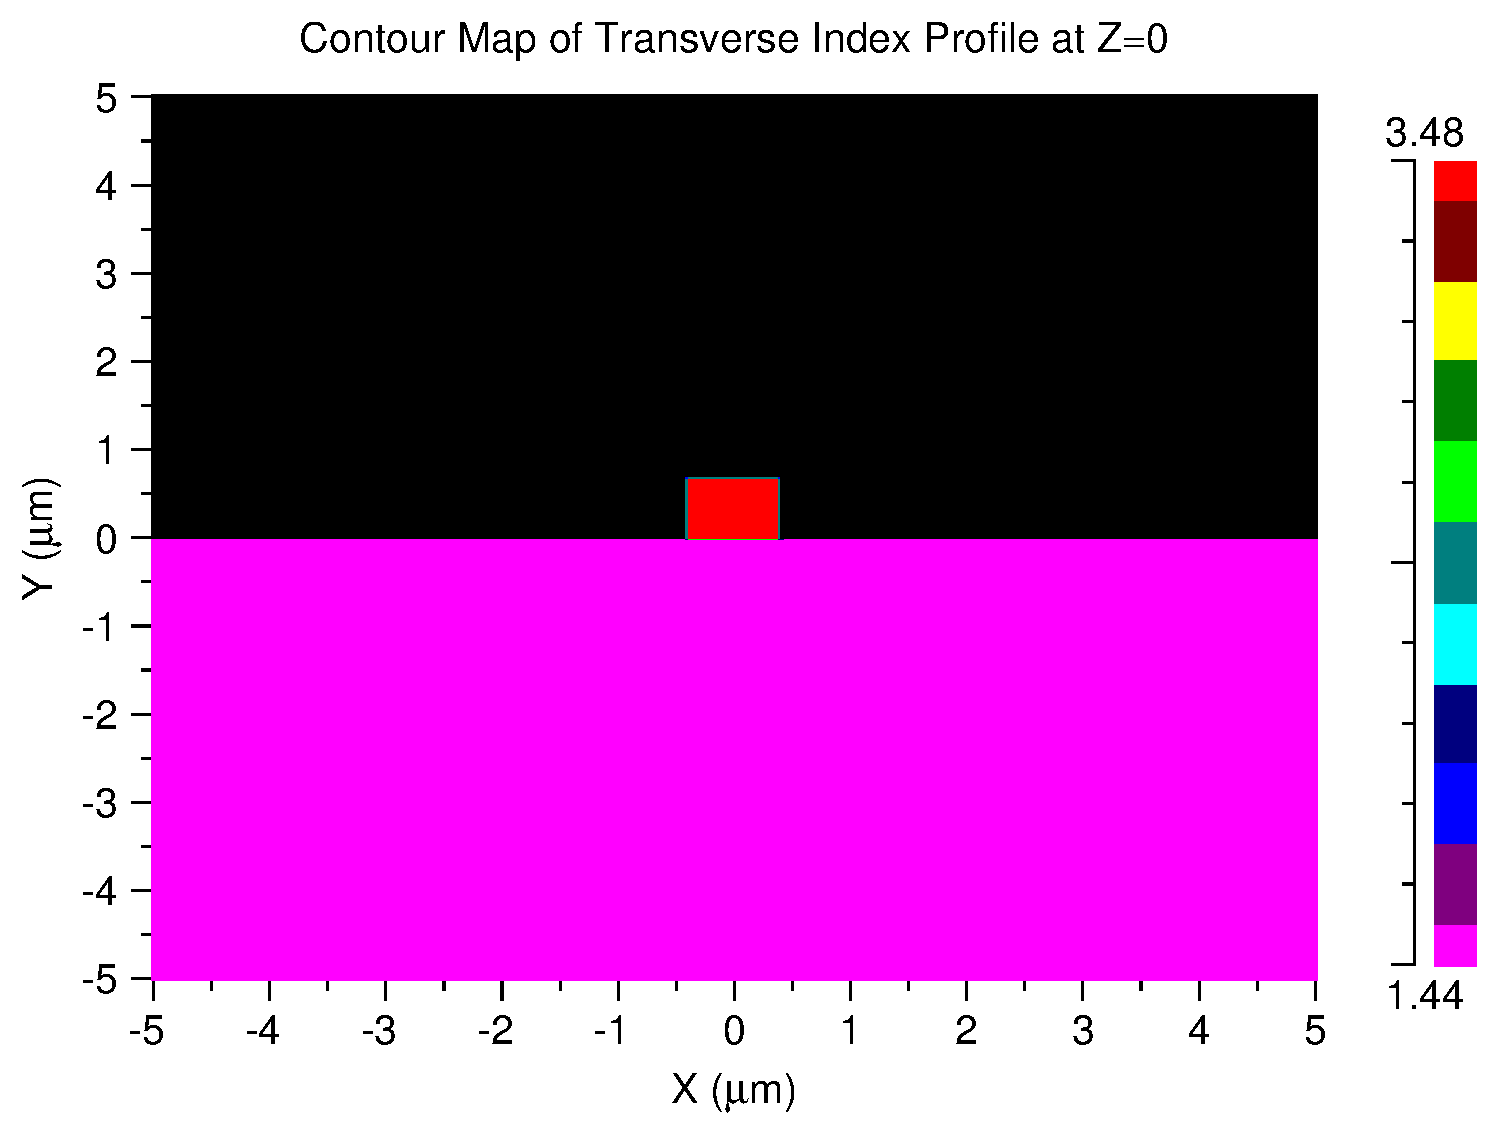
\includegraphics[totalheight=6 cm]{Grafiken/a3_index_profile.pdf}
\caption{}%
\label{fig:index_profile_3}%
\end{figure}


In the third task a silicon on insulator (SOI) strip waveguide of the length of $100~\upmu$m is simulated. The waveguide consists of a silicon core ($n=3.48$) with the height $h=0.7~\upmu$m and a width of $w=0.8~\upmu$m. This core is placed on a glass substrate ($n=1.44$). Above and on both sides of the waveguide there is air. This index profile is shown in \ref{fig:index_profile_3}. The gaussian exitation is shifted $0.25\cdot w$ in x-direction and $0.25\cdot h$ in y-direction, like in the task \ref{sec:task2}.

Next the TE and TM modes for $\lambda = 1.55~\upmu$m were calculated by using the correlation method. The field distribution of the calculated modes is shown in the figures \ref{fig:3TE} and \ref{fig:3TM}. The figures were named according to the nomenclature in the OWS lecture notes.

\begin{figure}%
\centering
%\begin{adjustwidth}{0cm}{0cm}
	\subfloat[HE$_{00}$  ]{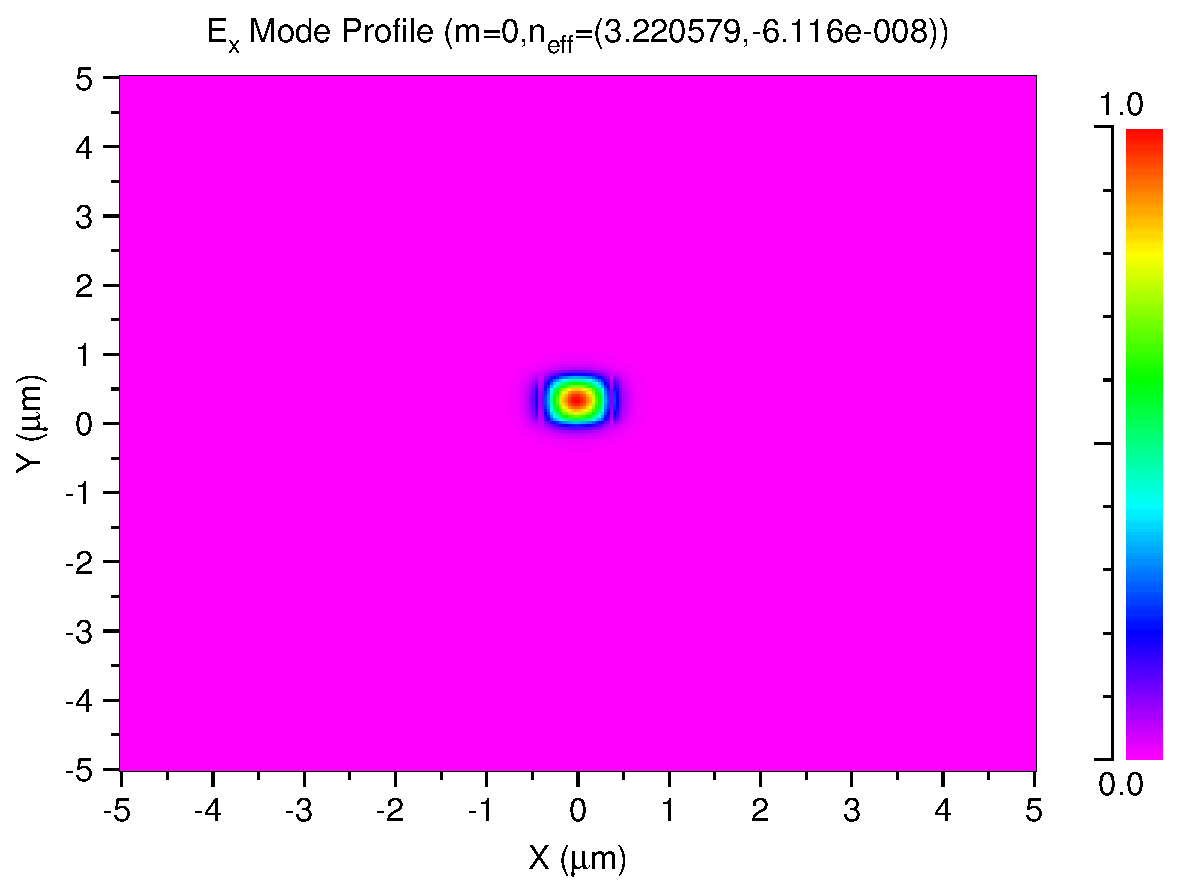
\includegraphics[totalheight=5 cm]{Grafiken/A3_TE_00.pdf}\label{fig:}}
	\subfloat[HE$_{10}$  ]{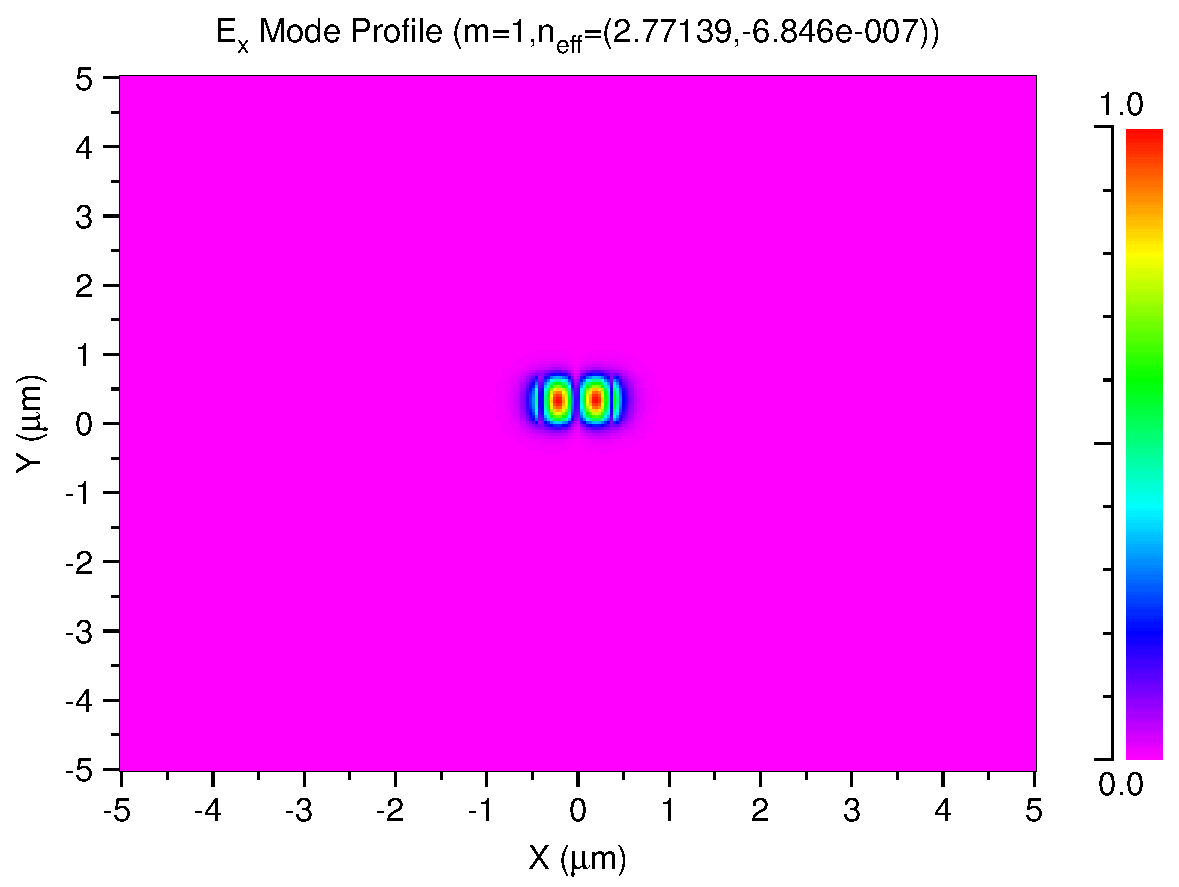
\includegraphics[totalheight=5 cm]{Grafiken/A3_TE_01.pdf} \label{fig:  }}\\%
	\subfloat[HE$_{11}$  ]{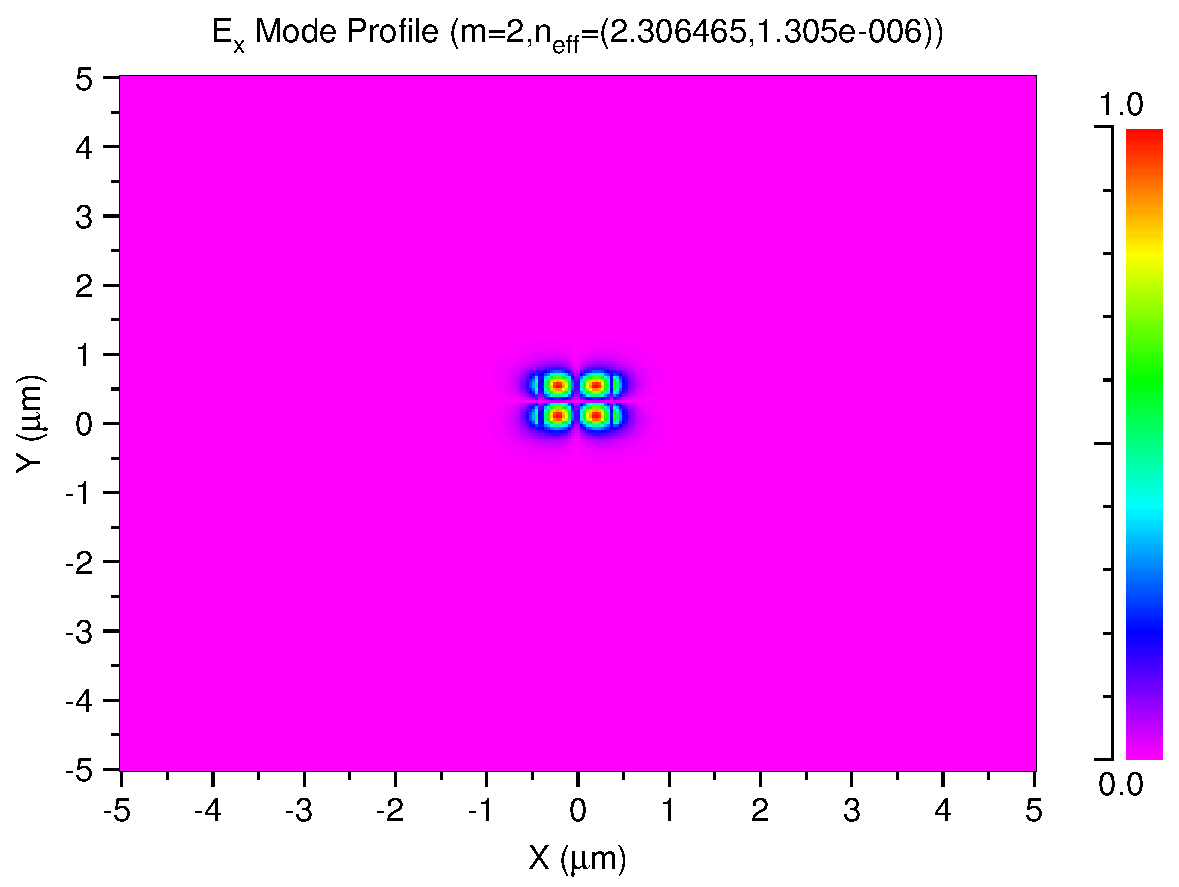
\includegraphics[totalheight=5 cm]{Grafiken/A3_TE_02.pdf}\label{fig:  }}
	\subfloat[HE$_{02}$  ]{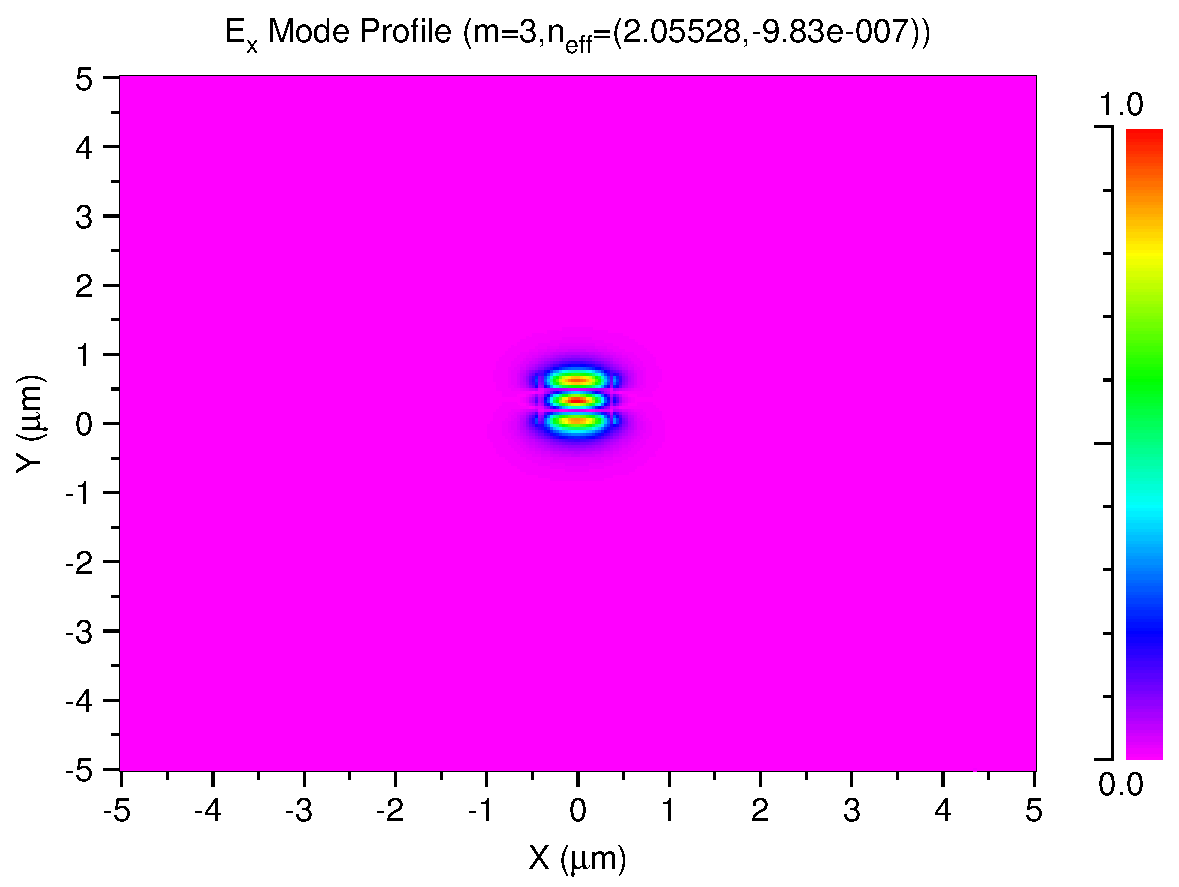
\includegraphics[totalheight=5 cm]{Grafiken/A3_TE_03.pdf} \label{fig:  }}\\
        \subfloat[HE$_{20}$  ]{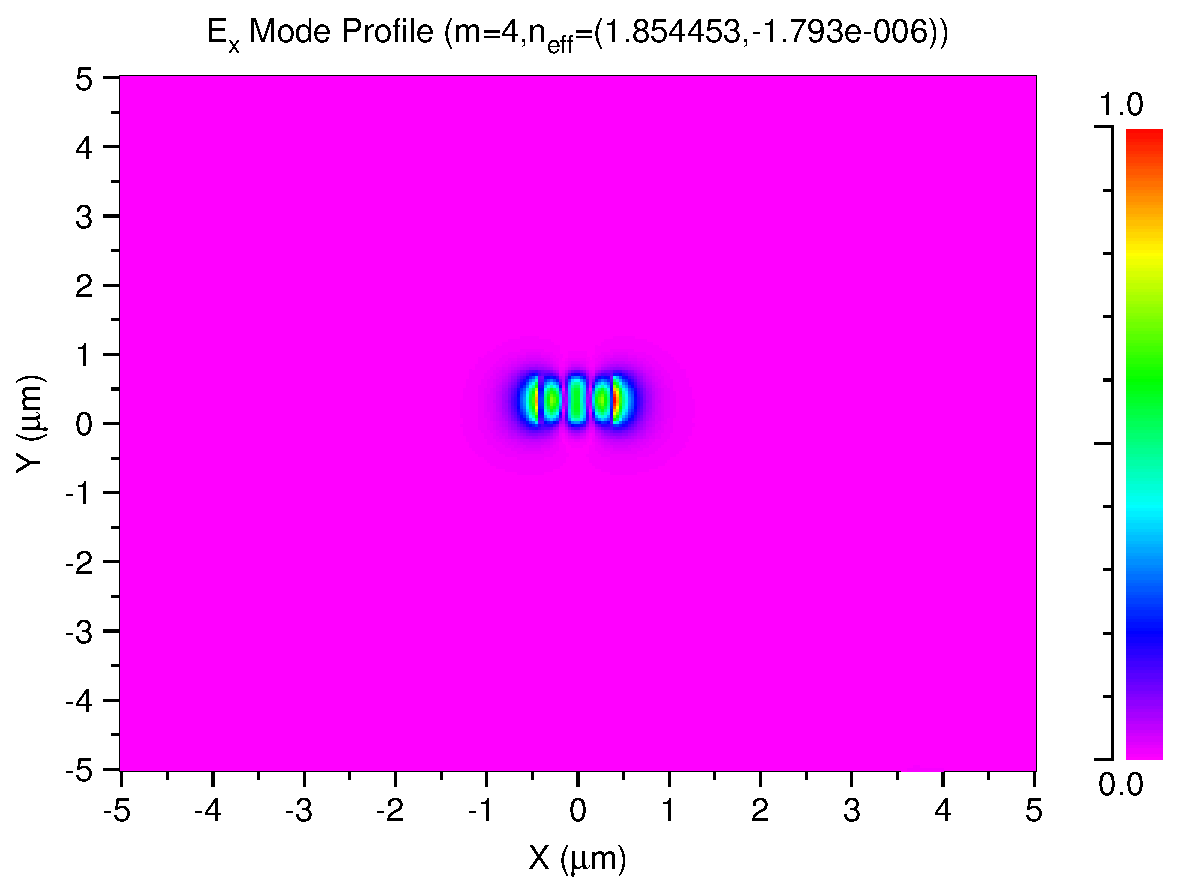
\includegraphics[totalheight=5 cm]{Grafiken/A3_TE_04.pdf}\label{fig:  }}
	\subfloat[not guided  ]{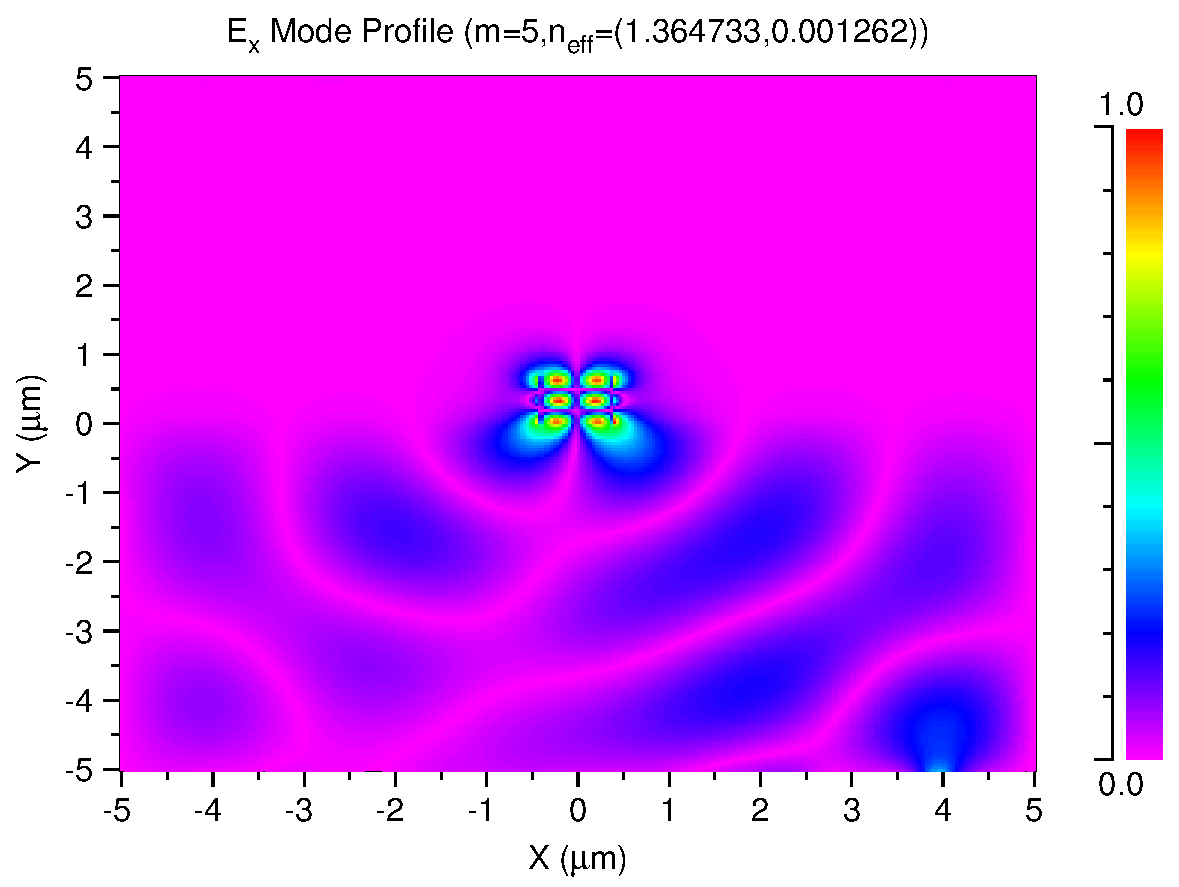
\includegraphics[totalheight=5 cm]{Grafiken/A3_TE_05.pdf} \label{fig:  }}\\
	\subfloat[not guided  ]{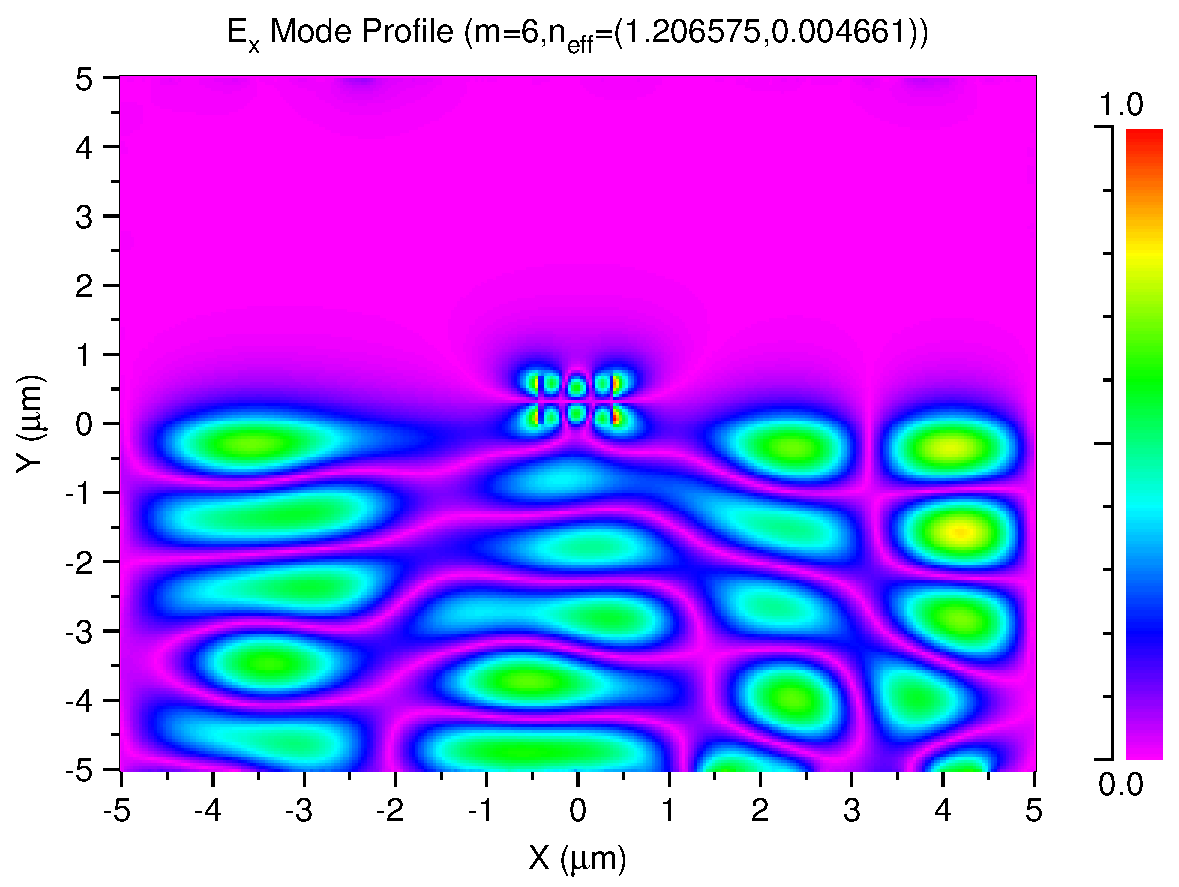
\includegraphics[totalheight=5 cm]{Grafiken/A3_TE_06.pdf}\label{fig:  }}
%\end{adjustwidth}
\caption{}%
\label{fig:3TE}%
\end{figure}

